\documentclass[12pt]{article}

\usepackage{amsmath}
\usepackage[utf8]{inputenc}
\usepackage[T1]{fontenc}
\usepackage[magyar]{babel}
\usepackage{graphicx}
\usepackage{float}
\usepackage[paper=a4paper,margin=1in]{geometry}

\usepackage{siunitx}
%%\title{%
%%  Kondenzált anyagok fizikája \\
%%  \large 1. Gyakorlat}
%%\author{}  
%%\maketitle


\begin{document}


\centerline{
\textsc{\Large{ Kondenzált anyagok fizikája}}
}
\centerline{ 
\textsc{\large{5. Gyakorlat}}
}
\vspace{10mm}

\textbf{Gy1.} Az  alábbi ábra az  FCC  kristályrácsú alumínium  pordiffrakciós képét  mutatja.  Az  egyes Debye-Scherrer gyűrűk alatt a mért
$2\theta$ szögek vannak feltüntetve. A beeső röntgensugárzás hullámhossza
 $\lambda= 2.02\AA$ volt. A mérési adatok alapján számítsuk ki az alumínium
a rácsparaméterét

\begin{figure}[h!]
\begin{center}
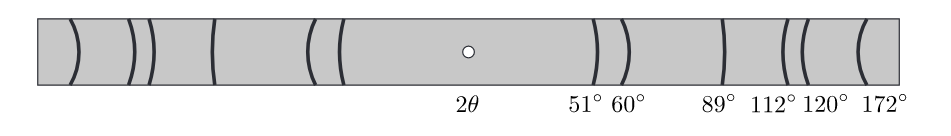
\includegraphics[height=2cm]{../images/Aldebyescherrer.png}
 \end{center}
\end{figure}

\textbf{Gy2.} A  grafén  olyan  kétdimenziós  anyag,  melynek  egyetlen  kristálysíkjában  a  szénatomok szabályos hatszögrácsban (honeycomb  lattice)  helyezkednek  el.  A  szomszédos  atomok  távolsága $a$.  Milyen
intenzitáseloszlást láthatunk  a  grafén  síkjával  párhuzamos, $L$
távolságra lévő  ernyőn, ha  merőlegesen $\lambda$ hullámhosszú röntgennyalábbal világítjuk  meg?  Vázoljuk  a z  intenzitáscsúcsok helyzeteit és magasságát!
\\

\textbf{Gy2.} Határozzuk meg az alábbi kristály primitív celláját és határozzuk meg a várható diffrakciós csúcsok relatív intenzitását a (h,k,l) paraméterek függvényében! Itt $f(\kappa)=1$ .
\begin{figure}[h!]
\begin{center}
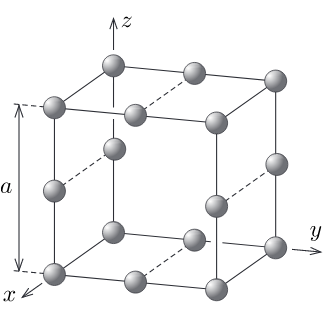
\includegraphics[height=6cm]{../images/5furakocka.png}
 \end{center}
\end{figure}

\end{document}